\documentclass[a4paper,landscape]{article}

\usepackage[landscape,top=0cm,left=0cm,bottom=0cm,right=0cm]{geometry}
\usepackage{tikz}
\usepackage{background}
\usepackage{blindtext}
\usetikzlibrary{matrix, shapes.misc, calc}

\pagestyle{empty}
\setlength{\parindent}{0cm}
\backgroundsetup{scale = 1, angle = 0, opacity = 1, color=black, contents = {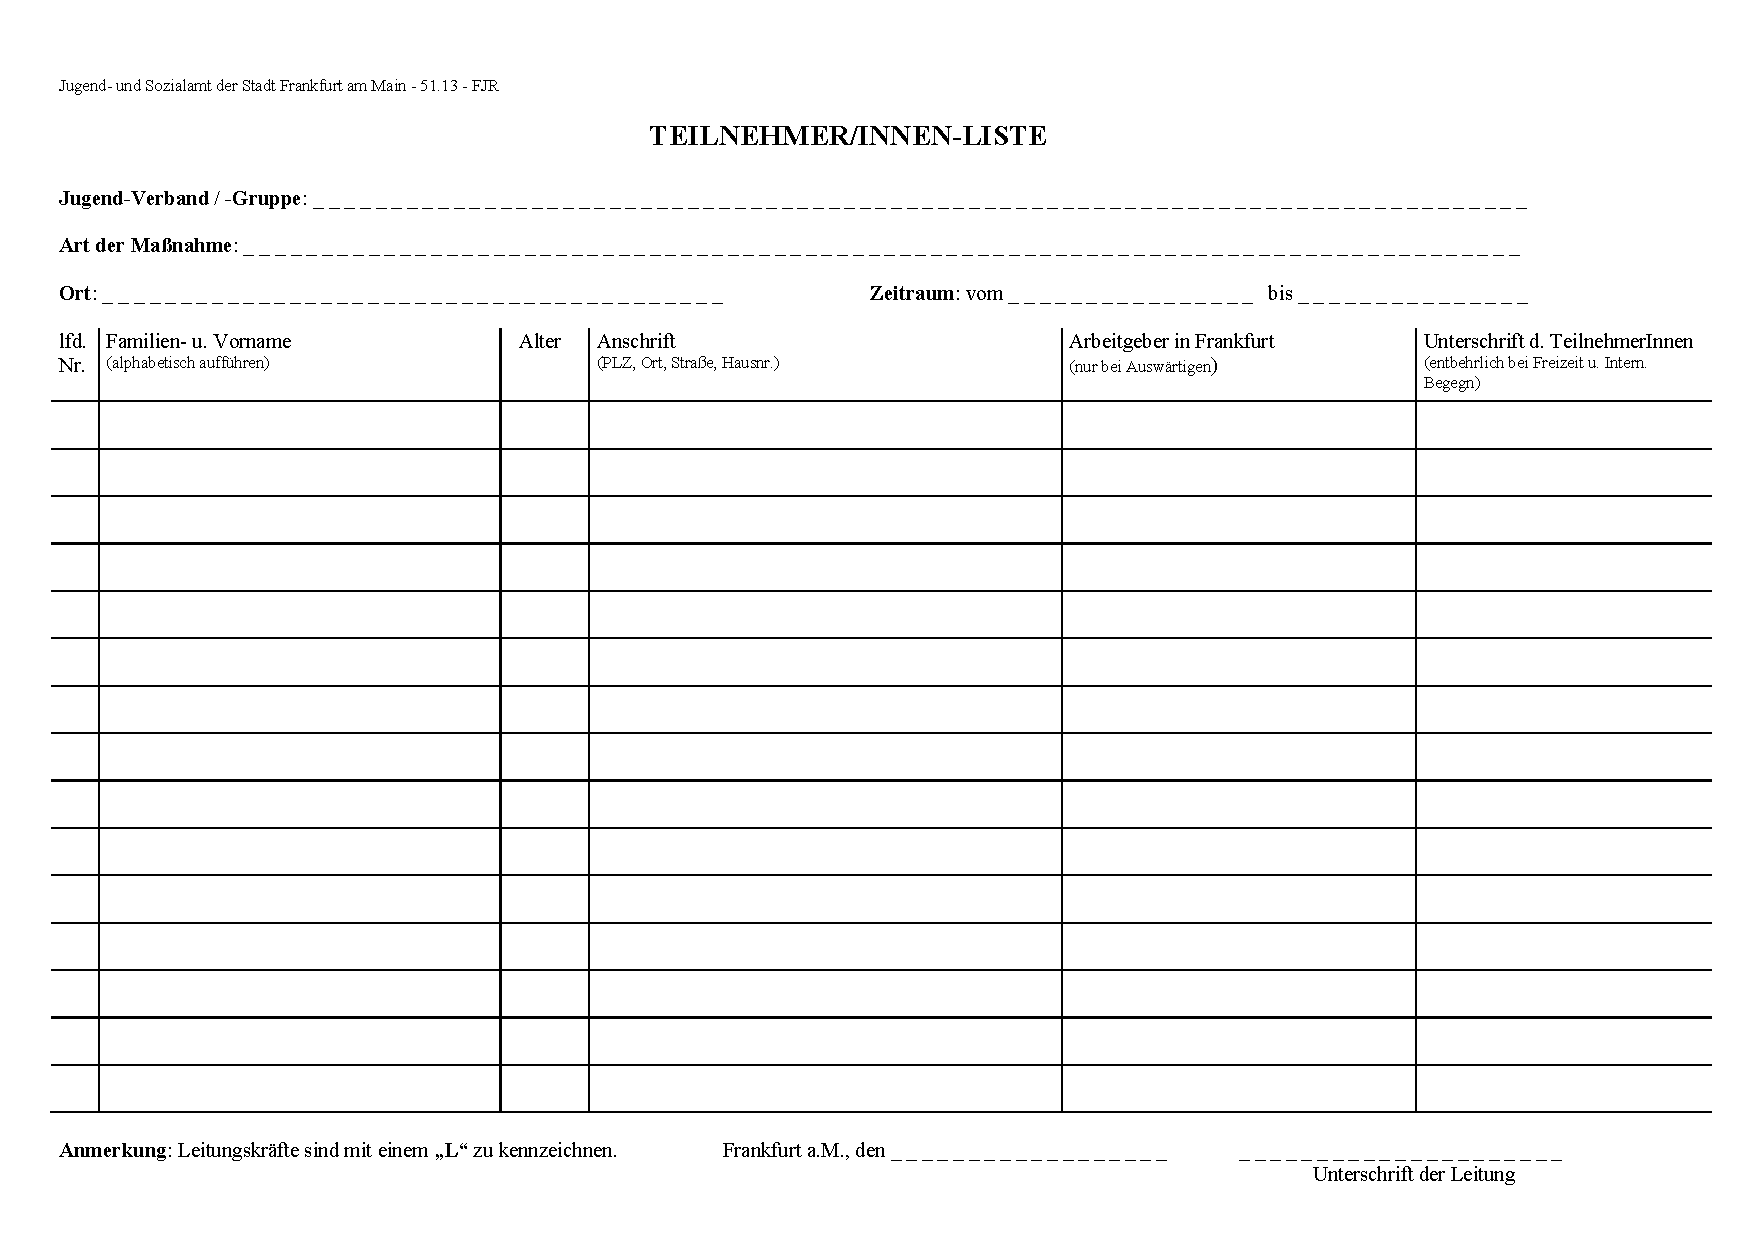
\includegraphics[width = \paperwidth, height = \paperheight] {city-frankfurt-main.pdf}}}

\begin{document}
\noindent \sffamily

@foreach($members as $chunk)
\begin{tikzpicture}[remember picture,overlay,yscale=-1]
    \node[anchor=base west] at (53.2mm,31.0mm) {\bfseries{\large{}}};   %Feld: Jugendverband/-Gruppe
    \node[anchor=base west] at (41.5mm,38.8mm) {\bfseries{\large{}}};   %Feld: Art der Maßnahme
    \node[anchor=base west] at (18.0mm,47.0mm) {\bfseries{\large{<<<!!$zipLocation!!>>>, <<<!!$countryName!!>>>}}};
    \node[anchor=base west] at (171.0mm,47.0mm) {\bfseries{\large{<<<!!$dateFromHuman!!>>>}}};
    \node[anchor=base west] at (220.0mm,47.0mm) {\bfseries{\large{<<<!!$dateUntilHuman!!>>>}}};

@foreach($chunk as $i => $member)
    \node[anchor=base, text width=4mm, align=center] at ($(8.0mm, 69.0mm + 8.05mm * <<<$i%15>>>)$) {<<<$memberShort($member)>>>};
    \node[anchor=base, text width=6mm, align=center] at ($(13.0mm, 69.0mm + 8.05mm * <<<$i%15>>>)$) {<<<$i+1>>>};
    \node[anchor=base, text width=67.5mm, align=center] at ($(50.65mm, 69.0mm + 8.05mm * <<<$i%15>>>)$) {<<<$memberName($member)>>>};
    \node[anchor=base, text width=14.6mm, align=center] at ($(92.2mm, 69.0mm + 8.05mm * <<<$i%15>>>)$) {<<<$memberAge($member)>>>};
    \node[anchor=base, text width=79.4mm, align=center] at ($(139.7mm, 69.0mm + 8.05mm * <<<$i%15>>>)$) {<<<$memberAddress($member)>>>};
@endforeach

\end{tikzpicture}

\pagebreak

@endforeach
\end{document}

